\chapter{Ontologies on the Web---putting it all together}
\label{ch14}

A comprehensive listing of ontologies in the wild is impossible, just as
a complete listing of all web pages is impossible. New ontologies and
open data sets on the Semantic Web are showing up every day. In Chapter~\ref{ch10}, we got a glimpse of the data sets that make up the data.gov project,
and we saw how data based on FOAF, Schema.org and OGP are scattered all over the
Web. In selecting ontologies for this chapter, we had to leave some
favorite projects behind.

We ended up with three examples. These examples were chosen for this
chapter because of their advanced use of modeling features beyond
RDFS-Plus, and how widespread their impact has been.


The first is called \emph{Quantities/Units/Dimensions/Types}, or QUDT for
short. It addresses an obvious problem that must be solved in any
attempt to align quantitative data, that is, measurement data from
multiple sources will be expressed in different units. In order to
integrate data, it is necessary to be able to determine whether two
quantities are commensurate (that's where the dimensions come in), and
if so, how to convert from one system to another (that's where the units
come in).

The second ontology is actually a whole collection of ontologies that are
collectively known as the \emph{Open Biological and Biomedical Ontologies}
(OBO). As the name implies, this is a set of ontologies about biological
and biomedical information.  OBO includes
massive amounts of data about biomedicine and biology, including genome
information, catalogs of known cancer genes, and biochemistry data.


The third is the \emph{Financial Industry Business Ontology} (\emph{FIBO} for short).
This is an ongoing effort by the Enterprise Data Management Council (EDMC) to 
build a reference ontology for the purpose of exchanging information about 
financial instruments.  It was inspired by
BCBS 239\cite{basel2013principles}, a white paper by the Based Commission 
on Banking Supervision, that outlined root causes for the financial crisis of
2008.  FIBO provides detailed logical definitions of financial instruments
for many purposes.  Its design is a good example of modeling for a very wide
audience of stakeholders. 


\section{Ontology Architecture}

Before we start talking about specific ontologies in OWL, we want to 
outline some of the facilities in OWL that help us manage ontologies and
the files we store them in.     Most software languages
have features for managing modularity of this sort, and OWL is no
exception.
These language features have no semantics for the model (i.e., they allow no
new triples to be inferred), but they help us, as humans, to organize a
model in a modular way.

There are many reasons why we might want to 
modularize our ontologies.  Some of them have to do with governance; if
I am responsible for changes to one part of an ontology, and you are 
responsible for changes to another, it might make sense to split them 
into two ontologies, so that each of us can change our own file without 
having to coordinate with the other.   Another reason has to do with 
the speed at which changes happen; if part of the ontology changes rapidly, 
and another part changes very slowly, we might want to split them out. 
As we'll see below, each of the examples in this chapter have made different
choices about how to modularize, but they all use the same features of OWL
to do it.  


\subsubsection{owl:Ontology}

OWL provides a built-in class whose members correspond to modular parts
of a semantic model. It is customary for the URI of an Ontology to
correspond to the URL of the file on the Web where the ontology is
stored. This makes use of a slightly different syntax in Turtle than we
have used so far. It is possible to spell out a URI by enclosing it in
angle brackets:

\begin{lstlisting}
<http://www.workingontologist.com/Examples/ch14/shakespeare.owl>
        a owl:Ontology.
\end{lstlisting}

Unlike the other constructs in OWL, the meaning of membership in
\texttt{owl:Ontology} is not given by inference. In fact, one could say that it
has no formal meaning at all. Informally, a member of \texttt{owl:Ontology}
corresponds to a set of RDF triples. The set of triples such a resource
corresponds to can be found by de-referencing its URI (as a URL), which
is expected (informally) to resolve to an RDF data set (e.g., an RDF
file). Formally, there is no connection in the model between an instance
of \texttt{owl:Ontology} and the triples to which it corresponds.

Although such an individual has no significance from the point of view
of model semantics, it can
be quite useful when specifying modularity of semantic models. The
primary way to specify modularity is with the property \texttt{owl:imports}.

\subsubsection{owl:imports}

This is a property that connects two instances of the class
\texttt{owl:Ontology}. Just as is the case with \texttt{owl:Ontology} itself, no
inferences are drawn based on \texttt{owl:imports}. But the meaning in terms of
modularity of models is clear: When any system loads triples from the
file corresponding to an instance of \texttt{owl:Ontology}, it can also find any
file corresponding to an imported ontology and load that as well. This
load can, in turn, trigger further imports, which trigger further loads,
and so on. There is no need to worry about the situation in which there
is a circuit of imports (e.g., if FIBO imports OGP imports FOAF imports FIBO).
A simple policy of taking no action when a file is imported for a second
time will guarantee that no vicious loops will occur. The resulting set
of triples is the union of all triples in all imported files.




\section{Quantities, Units, Dimensions and Types}
\label{QUDT}

As part of the Constellation Program, NASA developed an ontology 
(actually, several ontologies) to deal
with units of measure. The utility of controlling references to units in
science and engineering has been understood for centuries, and there are
several standard systems of units; there is the US Customary set of
units (with things like miles, feet, and degrees Fahrenheit), the
international system (``SI'') that includes meters, kilograms, and
Kelvins. NASA built an ontology of Quantities, Units, and Dimensions
(QUDT)\footnote{QUDT also includes information about Types, which is beyond the scope
of this treatment.}
to capture and manage this information.

What is the purpose of such an ontology? In contrast to OGP and Schema.org, 
which provide vocabularies that assist web page developers in
marking up their pages, QUDT cuts across many domains. It was designed
for science and engineering, but it has applicability in any setting
where information can be expressed in different units. We have already
seen an application for units in Schema.org (Example~\ref{Plushex}) 
---it is
important to know how a service is measured---by the hour, by the
minute, or by the job.

QUDT serves three major purposes in the Semantic Web. First, it provides
a global reference for units. If one information source says that some
product is measured in pounds, and another source
says that its service is provided in pounds, how do we know that they
are making reference to the same notion of pound (there is more than
one)? QUDT provides a URI for the notion of pound (with information to
distinguish it from other units with the same common name), so that such
references can be made unambiguously. QUDT is not alone in providing
this service; the United Nations maintains a standard called UN/CEFACT
which also  provides a canonical set of codes for unambiguously identifying
units. QUDT connects to the UN/CEFACT codes with the property
\texttt{qudt:uneceCommonCode}.

The second purpose that QUDT fills is to provide conversion services.
If two information sources
provide information in terms of pounds, and we use something like
UN/CEFACT or QUDT to determine that they are the same notion of pound,
then we can compare the offerings. But what if one of them offers a
product measured in pounds, and the other in kilograms? There are a few
things that have to happen before we can compare the offerings. First,
we have to understand whether it is even possible to compare pounds and
kilograms (are they ``commensurate'' values?). If they are, then we need
to convert values from one unit to the other. QUDT offers both of these
services. These services are useful in science and engineering settings,
but also in more common settings like the commercial applications of
Schema.org. 

The third purpose that QUDT serves is mostly focused on engineering
settings, where it is often important to verify the dimensions of
certain quantities. One way to check for errors in a formula is to check
the dimensions of the components of a formula; only quantities with the
same dimensions may be added to one another or compared to one another;
for example, it makes no sense to add kilograms to centimeters or to
compare seconds to feet. A simple check for correct dimensions can turn
up errors, even in quite complex formulas. QUDT includes a comprehensive
model of dimensions, cross-referenced with units, which enables
dimension-based calculations. The simplest application of this facility
is for units conversion---it makes no sense to convert from one unit to
another, if the units don't have the same dimension. The formula to
convert from meters to feet, 1m = 3.28 ft, can be checked for
dimensional correctness---do meters and feet have the same dimension?
Yes, they do; both are measures of \emph{length}.

We will explore just enough of the QUDT ontology to show how it supports
these three functions. The QUDT ontology supports this functionality
through a careful separation of Quantities, Units, and Dimensions. In
some sense, there is nothing new about this separation; treatment of
these things has been ongoing in science and engineering for centuries.
QUDT makes it referenceable on the Web and actionable. Further
information about QUDT can be found at its web site, QUDT.org.

A \emph{Quantity} is some measurable property. A \emph{Quantity Kind} is,
appropriately enough, the kind of thing one can measure---familiar
quantity kinds are length, time, mass, and force, etc. A \emph{Unit} is a
standard of measurement for a particular quantity kind. A foot is a unit
for measuring length; a second is a unit for measuring time. It is
common to have several units for a single kind; feet, inches,
kilometers, Angstroms, light-years, and furlongs are all measures for
length.

QUDT uses the \emph{Local Restriction of Range} pattern described in Section~\ref{lror}; that is, it uses
\texttt{owl:allValuesFrom} to restrict the possible values for a property. The
relationship between \texttt{qudt:Unit} and \texttt{qudt:QuantityKind} is called
\texttt{qudt:hasQuantityKind} (note the naming convention; \texttt{qudt:hasQuantityKind} begins
with a lower-case letter, and hence is a property; \texttt{qudt:QuantityKind}
begins with an upper-case letter and is a class). The restriction on
this relationship is defined as

\begin{lstlisting}
qudt:Unit a owl:Class ;
  rdfs:subClassOf [
      rdf:type owl:Restriction ;
      owl:allValuesFrom qudt:QuantityKind ;
      owl:onProperty qudt:hasQuantityKind ;
    ] ;
qudt:hasQuantityKind a owl:ObjectProperty .
qudt:QuantityKind a owl:Class .
\end{lstlisting}


As an example of units and quantity, let's have a look at feet and
length:

\begin{lstlisting}
unit:FT a qudt:Unit ;
      qudt:hasQuantityKind hasQuantitykind:Length .
\end{lstlisting}

Following along as in the example of this pattern from Section~\ref{lror}, from
these triples we can infer that

\begin{lstlisting}
quantitykind:Length a qudt:QuantityKind .
\end{lstlisting}

QUDT includes a comprehensive list of units and quantity kinds from many
fields of science, including mechanics, thermodynamics, chemistry,
informatics, and biology. It organizes its namespaces in a modular
way---as we saw in this example, resources that describe how units work
(like the resources \texttt{qudt:QuantityKind} and \texttt{qudt:Unit}) are in the \texttt{qudt:}
namespace, while particular quantities and units (like
\texttt{quantitykind:Length} and \texttt{unit:FT}) are in specific namespaces
for quantity kinds and units, respectively. 
These resources resolve the first function of the QUDT vocabulary, that
is, they provide unambiguous reference URIs for all the units and
quantity kinds in QUDT.

\subsection{Converting Units with QUDT}

QUDT includes information that can be used to convert measurements from
one unit to another. This is a workhorse for merging quantitative
information on the Semantic Web. Conversions can be within the same
system of units (meters to kilometers, seconds to hours, feet to miles)
or crossing between systems (miles to kilometers, degrees Fahrenheit to
degrees Centigrade). In order for such a conversion to make sense, the
units must be commensurate---that is, they measure the same kind of
thing. Miles and kilometers are both measurements of length, so it makes
sense to consider a conversion between the two. Seconds and degrees
Fahrenheit do not measure the same thing; it is not meaningful to
convert from one to another.

In QUDT, we can tell if two units are commensurate if they measure the same
kind of quantity.  This is represented in QUDT with a \texttt{QuantityKind}.  
This means that we can query for whether two units, say feet and meters,  are commensurate with
the following SPARQL
query:

\begin{query}Finding commensurate units \end{query}
\begin{lstlisting}
ASK WHERE {
     unit:M qudt:hasQuantityKind ?kind .
     unit:FT qudt:hasQuantityKind ?kind .
}
\end{lstlisting}


%That is, \texttt{?arg1} and \texttt{?arg2} are commensurate, if their associated quantity
%kinds are related to a common ancestor in the \texttt{qudt:generalization} tree.
%Recall that \texttt{qudt:generalization}* will match zero or more repeated
%ccurrences of \texttt{qudt:generalization}, so that if there is a single value for  \texttt{?kind} 
%for both arguments (e.g,. Length), they will match; this means that the query
%will return true for \texttt{?arg1} bound to \texttt{unit:FT} (foot) and \texttt{?arg2} bound to
%\texttt{unit:M} (meter). It will also return true for
%\texttt{vocab-quantities:PotentialEnergy} and \texttt{vocab-quantities:ThermalEnergy},
%because they both have a common generalization,
%\texttt{vocab-quantities:EnergyAndWork}.

Once we have determined that two units are commensurate, we can set
about converting measurements in one unit to the other. Each unit
includes two properties---\texttt{qudt:conversionMultiplier} and
\texttt{qudt:conversionOffset}. As their names suggest, these provide conversion
multipliers and offsets for each unit. For each dimension, there is a
base unit for which the multiplier is 1 and the offset 0. It isn't
important to know what the base unit is, in order to convert from one
unit to the other. For example, to convert ten kilometers to miles, we
can use the query

\begin{query}Converting 10 kilometers to miles\end{query}
\begin{lstlisting}
SELECT (((((?val * ?M1) + ?O1) - ?O2) / ?M2) AS ?converted)
WHERE {
    BIND (10.0 AS ?val)
    unit:KM qudt:conversionMultiplier ?M1 ;
              qudt:conversionOffset ?O1 .
    
    unit:MI qudt:conversionMultiplier ?M2 ;
            qudt:conversionOffset ?O2 .
}
\end{lstlisting}


Answer: \textbf{6.2137119223733395}

QUDT includes over five hundred conversion factors, enabling thousands
of such conversions.

\subsection{Using QUDT conversions}

We can express these conversions in a SPARQL query, but this isn't
available as an inference. That is, if we have some quantity specified
in miles, we can't always count on an inference engine to express that
value in kilometers. Calculations of this sort are the sort of things
that one usually puts into an application program. SHACL Rules
(Section~\ref{shacl-rules}) is an example of
how to make these conversions into inferences.  
We already saw how SHACL-Rules can  be used to
attach queries to an ontology. Here we see another application of SHACL-Rules.
The query we used to convert kilometers to miles required us to put the
information about the conversion into the query; the number to be
converted (10.0), the source unit (kilometer), and the target unit
(mile). If we want to do another conversion, we would need another
query, very similar in form, but with a different measurement and
different designations of units. Far more convenient would be to
parameterize the query, making it effectively into a function
definition. The generalized query, using variables ?arg1, ?arg2, etc.,
for the function arguments, looks like

\begin{query}Parameterized conversions\end{query}
\begin{lstlisting}
SELECT (((((?arg1 * ?M1) + ?O1) - ?O2) / ?M2) AS ?value)
WHERE {
    ?arg2 qudt:conversionMultiplier ?M1 ;
    qudt:conversionOffset ?O1 .
    ?arg3 qudt:conversionMultiplier ?M2 ;
    qudt:conversionOffset ?O2 .
}
\end{lstlisting}


SHACL extensions \cite{Steyskal:17:SAF} allow such queries to be given names, 
which themselves are
resources in RDF.   When we do this, we refer to the named query 
as a \emph{function}.  If we give this query the 
name \texttt{qudtsh:convert}, then
we could write the 10 kilometer query simply as

\begin{query}
\begin{lstlisting}
SELECT (qudtsh:convert(10.0, unit:KM, unit:MI)
                   AS ?value)
WHERE {}
\end{lstlisting}
\end{query}

Answer: 6.21

The call to the function \texttt{qudtsh:convert} is doing all the work---there is
nothing in the
WHERE clause to match at all!

The conversion of 32 degrees Fahrenheit to Centigrade looks very
similar:

\begin{query}Convert Fahrenheit to Celsius\end{query}
\begin{lstlisting}
SELECT (qudtsh:convert(32.0, unit:DEG_F,
unit:DEG_C)
AS ?value)
WHERE {}
\end{lstlisting}


Answer: 0.0

\begin{challenge}{Comparison Shopping with Good Relations}
\label{chal:38}

Now that we can use QUDT to convert values from one unit to another, we
can apply this to Schema.org data for purposes of comparison
shopping.

In Example~\ref{Plushex}, we have an example of a massage
service, priced at \$80.00 for an hour and a half session (see Figure~\ref{fig:ch10.plushdata})

Down the street from Plush, the Style Cafe, a competing day spa, has 
its own offer---a
fifteen-minute chair massage, for the busy person-on-the-go:

\begin{lstlisting}
style:StyleCafe
  a schema:DaySpa ;
  schema:makesOffer style:Offer10 .
style:Offer10
  rdf:type schema:Offer ;
  schema:priceSpecification style:PriceSpec10 ;
  schema:includesObject style:ChairMassage ;
  rdfs:label "Chair massage" .
style:PriceSpec10
  rdf:type schema:UnitPriceSpecification ;
  schema:price "15.0" ;
  schema:priceCurrency "USD" .
style:ChairMassage
  a schema:TypeAndQuantityNode ;
  schema:amountOfThisGood "15" ;
  schema:unitCode unit:MIN ;  
  schema:typeOfGood style:Massage .
\end{lstlisting}



Suppose we want to compare these two offerings in terms of their price
per minute of services. All the information is there---one of them costs
\$15 for 15 minutes, the other is \$80 for an hour and a half. But to
make the comparison, we have to convert the amounts into the same units.

We can do this by combining Schema.org with QUDT. First, we want to
query the Schema.org data to find out all the things we need to know
to make the comparison. We can do this simply by generalizing the common
data form into a query:

\begin{query}Combining Services for Comparison\end{query}
\begin{lstlisting}
SELECT * 
WHERE {
?spa a schema:DaySpa ;
  schema:makesOffer ?offer .
?offer a schema:Offer ;
  schema:priceSpecification ?pricespec ;
  schema:includesObject ?tqn ;
  rdfs:label ?offering .
?pricespec a schema:UnitPriceSpecification ;
  schema:price ?price ;
  schema:priceCurrency ?currency .
?tqn a schema:TypeAndQuantityNode ;
  schema:amountOfThisGood ?duration ;
  schema:unitCode ?qunit ;  
  schema:typeOfGood plush:Massage .
}
\end{lstlisting}

The graph pattern (the part after the keyword WHERE) corresponds line
per line to the data, with all the values that the two examples don't
have in common turned into variables. We have chosen names for the
variables that indicate their role in the graph; for example, \texttt{?pricespec}
is a \texttt{UnitPriceSpecification}; \texttt{?qunit} refers to the QUDT units.

Now we can use QUDT to compute a comparable cost rate in price per
minute. The choice of ``minutes'' here is somewhat arbitrary---we could
have as easily chosen any other time unit, like seconds or hours. Now
that we know what units (?qudtunit) the amount (?amt) is in, we can
convert it to minutes using \texttt{qudtsh:convert}:

\begin{lstlisting}
qudtsh:convert (?amt, ?qudtunit, unit:MIN)
\end{lstlisting}

We can compute the cost per minute by dividing \texttt{?price} by this. The final
query is

\begin{query}Price comparison of two services\end{query}
\begin{lstlisting}
SELECT ?offering ?currency ?cost_per_min
WHERE {
?spa a schema:DaySpa ;
  schema:makesOffer ?offer .
?offer a schema:Offer ;
  schema:priceSpecification ?pricespec ;
  schema:includesObject ?tqn ;
  rdfs:label ?offering .
?pricespec a schema:UnitPriceSpecification ;
  schema:price ?price ;
  schema:priceCurrency ?currency .
?tqn  a schema:TypeAndQuantityNode ;
  schema:amountOfThisGood ?duration ;
  schema:unitCode ?qunit ;  
  schema:typeOfGood plush:Massage .
BIND ((?price/qudtsh:convert(?duration, ?qunit,
                             unit:MIN)) AS ?cost_per_min )
    }
ORDER BY ( ?cost_per_min )
\end{lstlisting}

Answer:

\begin{tabular}{|lll|}
\hline
servicename&currency&cost\_per\_min\\
\hline
Relaxing Massage&USD&0.88\\
Chair Massage&USD&1.0\\
\hline
\end{tabular}

We have given the quotient of price per minute the name \texttt{?cost\_per\_min},
and sorted from lowest cost to highest. The result shows that the
Relaxing Massage is the better value per minute.
\end{challenge}

This example shows a number of features of the role that models play in
linking data sources. The structure of Schema.org gave
us a consistent way to represent offerings, prices, amounts, and units
of competing businesses. QUDT provides useful services (units
conversions) for computations over these data. Schema.org allows our 
descriptions to refer to external sources (in this case, QUDT) to define
its details, making it easy to connect the two offerings. 

\subsection{Dimension Checking in QUDT}

There are a lot of services that an engineer or scientist could ask of a
system of units; many of these go by the name \emph{dimensional analysis}.
Whole books have been written on the subject; we can barely scratch the
surface of this topic here (therefore, see the Further Reading section
at the conclusion of the book). We will illustrate enough of the QUDT
ontology to show how it can support certain basic operations in
dimensional analysis.

The basic idea of dimensional analysis is that a quantity kind has a
signature that tells how it relates to
basic dimensions like length, time, and mass. QUDT defines eight base
dimensions of this sort, but in this exposition, we will focus on these
three. A compound quantity kind has a signature in these basic dimensions.
For example, the compound quantity kind \emph{velocity} is defined as a ratio
between distance and time; this means that its signature in terms of
length, time, and mass is length/time. The signature can be written as a
vector, with one vector component for each base unit, and the magnitude
of the vector in that component being the exponent of the base quantity
in the formula for the compound quantity. If we write our vectors in the
order {[}length, mass, time{]} then the vector for velocity is {[}1, 0,
-1{]}. The vector for any base quantity will have magnitude 1 in exactly
one place; so the vector for mass is {[}0, 1, 0{]}. Acceleration is
given as a quotient of velocity by time; so its vector is {[}1, 0,
-2{]}.

This vector is called the \emph{dimensionality} of a compound unit. These
vectors can be used to check the validity of a scientific or engineering
formula. For example, one of the basic laws of motion is given by the
formula F = ma, or Force equals the product of mass times acceleration.
Only quantities with identical dimensionality can be meaningfully
compared, so this formula makes sense only if the dimensionality of
Force is the same as the dimensionality of the product of mass and
acceleration. The dimensionality of Force is given by the expression
$ml/{t^2}$ , that is, mass times length divided by time twice. The
dimensionality of acceleration is given as $l/{t^2}$, or length divided by
time twice, and mass is given simply by $m$. So we can check the
dimensionality of $F = ma$ by replacing each term with its dimensions,
i.e., ${ml}/{t^2} = m(l/{t^2})$. Since the dimensions on both sides are the
same, the formula has been verified to pass the test of dimensionality.
It is important to note that this kind of simple dimensional analysis
can uncover certain formulas that are incorrect; a correct dimensional
analysis does not guarantee that the formula doesn't have some other
problems with it.

In terms of dimension vectors, we can do the same calculation using
vectors. The dimension vector for force is $[1, 1, -2]$. The vector
for mass is $[0, 1, 0]$ and the vector for acceleration is $[1, 0,
-2]$. The formula is verified if the vectors add up; that is, if the
vector for mass plus the vector for acceleration
equals the vector for force. We add vectors element by element, and
verify that indeed $[0, 1, 0] + [1, 0, -2] = [1, 1, -2]$, verifying that the dimensions of the
formula are identical.


\begin{figure}
\centering
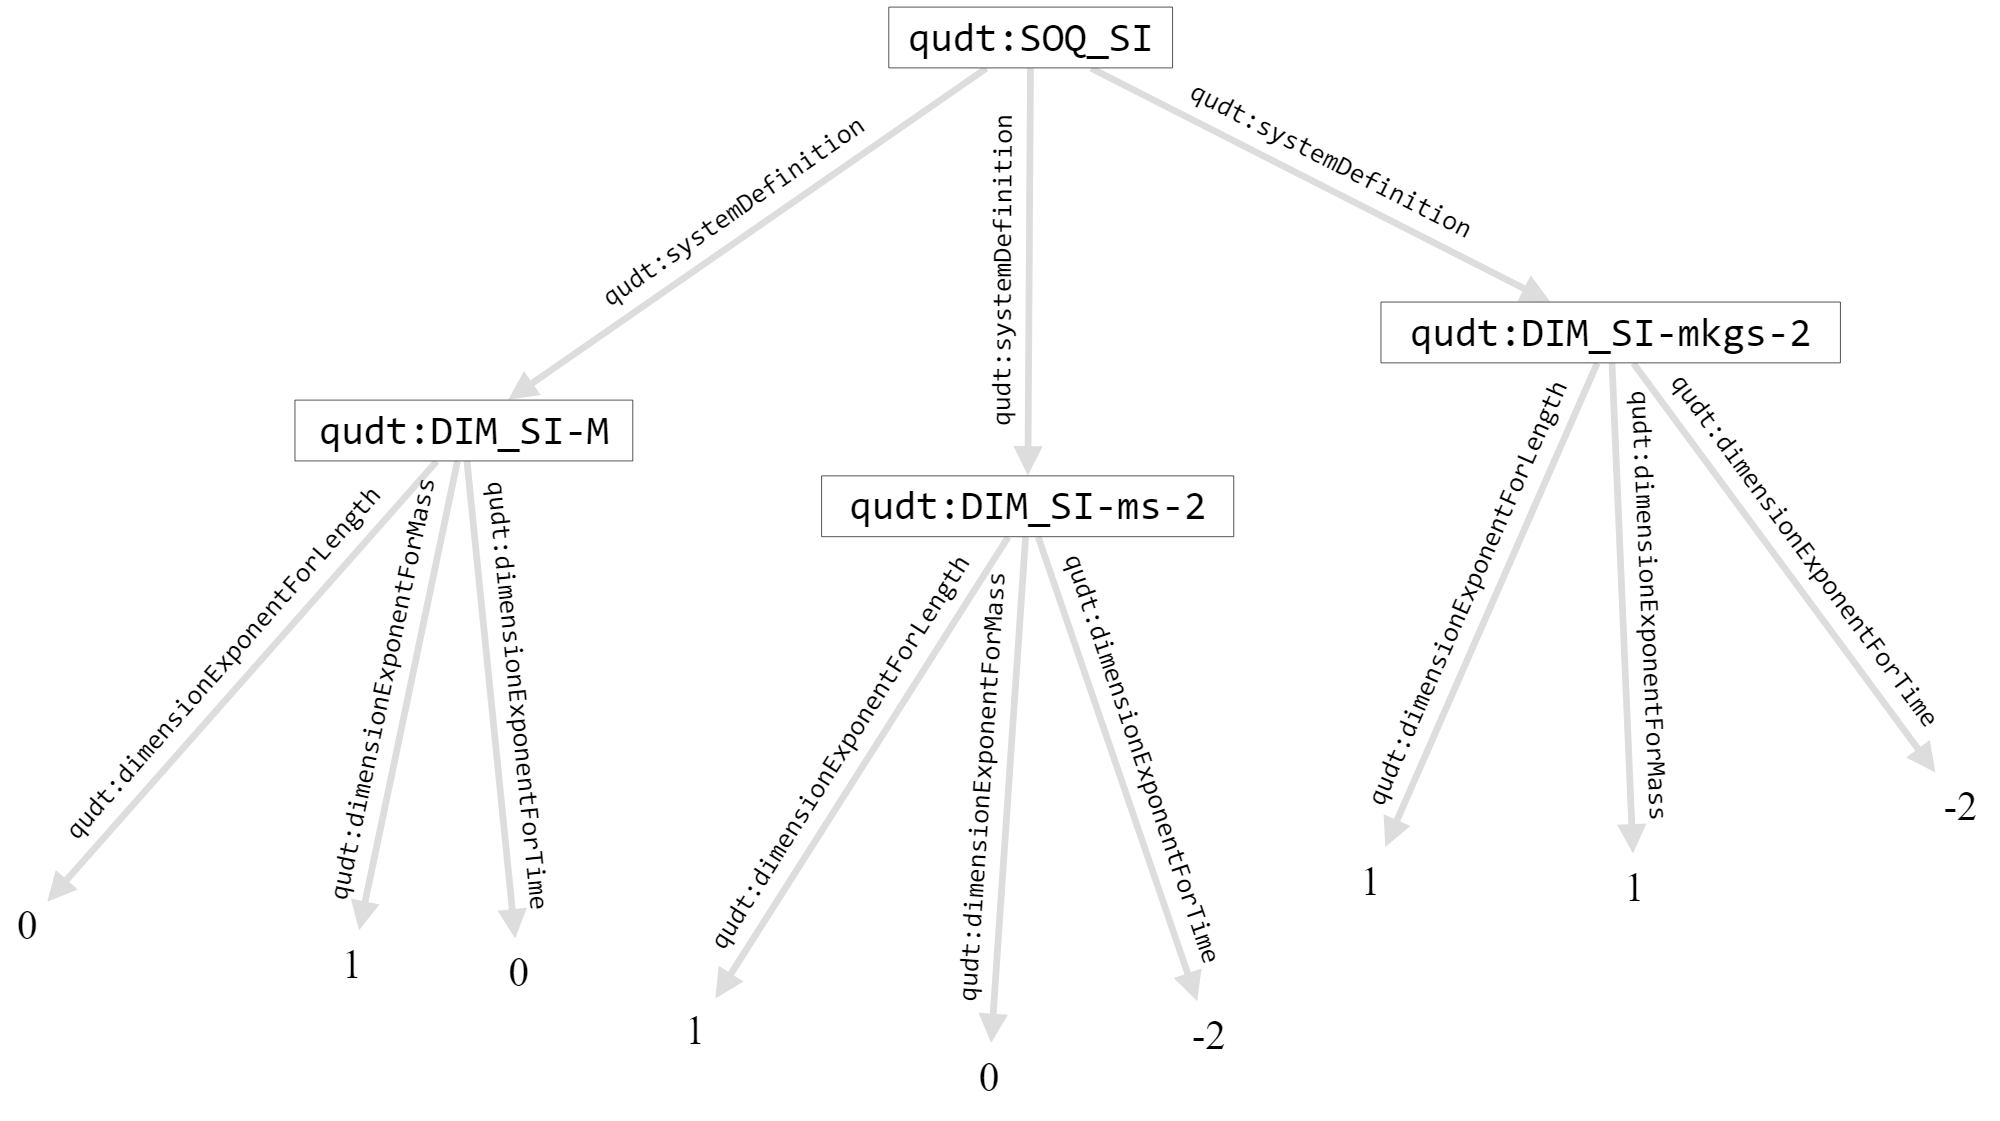
\includegraphics[width=5in]{SWWOv3/media/ch14/figure14-1.png}
\caption{Dimensional structure in QUDT to support analysis of $F=ma$ (time
dimension)}
\label{fig:ch14.04}
\end{figure}






QUDT supports dimensional analysis by representing over 200 dimension vectors,
cross-referenced with corresponding quantity kinds, each organized in a 
form analagous to what you see in Figure~\ref{fig:ch14.04}.

First, there is the \emph{System of Quantities}, or, more precisely, \emph{System of Quantity Kinds} . QUDT includes eight different
systems of quantity kinds, including the standard international (``metric'')
system (SI, shown in the figure) as well as several variants of the CGS
(centimeter-gram-second) and the US Customary system (with inches,
yards, miles, pounds, etc.). A system of quantity kinds defines the
dimensions that can be measured in that system. Each system typically
has dozens of dimension vectors associated with it. In the figure, we see three
dimension vectors associated with the SI system of quantities---one for mass
(\texttt{DIM\_SI-M}), one for length over time twice (\texttt{DIM\_SI-ms-2})
and one for length times mass over time twice (\texttt{DIM\_SI-mkgs-2}).
The naming convention for these dimension vectors includes the name of the
system (SI) followed by the dimensions in the order length, mass, time,
each followed by a number indicating the exponent for that dimension.
These names are not used by any query mechanism---they are only used for
humans to read the dimension names.

Since the names are only there for humans to read, if we want to query
for the dimension vector for any of these, we need to represent their
dimensional vectors in triples.  QUDT represents these in many ways for 
different use cases, but for this example, we'll just use the simplest 
one, as shown in Figure~\ref{fig:ch14.04}.  Each base dimension (Length, Mass and Time) has a particular
property associated with it, which indicates the coefficient.  The names for 
these properties are very specific and descriptive; for example, the property that indicates
the exponent for mass in a particular dimension is called \texttt{qudt:dimensionExponentForMass}. Similar properties 
are used to indicate exponents for other dimensions. 

From the information in Figure~\ref{fig:ch14.04}, 
we are in
a position to verify  that the formula $F = ma$ 
is correct from a dimensional point of view, by noticing that for each base 
dimension, Mass, Length and Time, 
the coefficient for the quantity vectors in the formula add up; the coefficent for mass (0) plus that for linear acceleration (-2)
equals the coefficient for force (-2); $0 + (-2) = -2$.

How can we write a SPARQL query to verify this calculation?  Let's start by 
looking at just one dimension, say Time.  We need to get the coefficient for each
term in the formula for the Time dimension:

\begin{query}Time dimension for each term\end{query}
\begin{lstlisting}
SELECT ?term ?val
WHERE { 
     VALUES ?term {qudt:DIM_SI-M
                   qudt:DIM_SI-ms-2 
                   qudt:DIM_SI-mkgs-2 
                  }
        ?term qudt:dimensionExponentForTime ?val .
    } 
\end{lstlisting}

Notice that we used the \texttt{VALUES} construct from Section~\ref{sparqlvalues} to 
list the terms in the formula.  

So far, we have not indicated which side of the equal sign they
are, so we can't sensibly add them up.  We want to add up all the 
values on one side of the equation and subtract the values from the other;
so we need to do two things.  First, to indicate which side each term is on,
then multiply the values on one side by $-1$ before we add them up to 
compare to zero.   

We can use the more extended form of VALUES to indicate which side of the 
formula they are on, and use a BIND statement (with an IF function) to 
multiply just one set of them by $-1$.  Then we want to add them up to 
see what the total exponent is. 

\begin{query}Balanced sum of Time exponents\end{query}
\begin{lstlisting}
SELECT (SUM(?val) AS ?formtotal)
WHERE { 
     VALUES (?term ?side) {(qudt:DIM_SI-M :left)
                           (qudt:DIM_SI-ms-2  :left)
                           (qudt:DIM_SI-mkgs-2 :right)
                  }
        ?term qudt:dimensionExponentForTime ?exp .
        BIND (IF (?side=:right, -1*?exp, ?exp) AS ?val)
    } 
\end{lstlisting}

Now, we want to do this for every dimension.  In the Semantic Web, properties
are just as important as classes; we can represent the dimensions in the 
analysis by the three properties that represent the exponents for the three 
dimensions we are working with.  

We can use VALUES again, separately from the first, so that we get all combinations 
of dimensions and terms.  We have to GROUP BY the dimension, so that we only add up
exponents in a single dimension. 

\begin{query}Total exponents in each dimension\end{query}
\begin{lstlisting}
SELECT ?dim (SUM (?exp) AS ?formtotal)
WHERE {VALUES ?dim {qudt:dimensionExponentForLength 
                 qudt:dimensionExponentForTime 
                 qudt:dimensionExponentForMass}
     VALUES (?term1 ?side) {(qudt:DIM_SI-M :left)
                            (qudt:DIM_SI-ms-2 :left)
                            (qudt:DIM_SI-mkgs-2 :right)
                           }
        ?term1 ?dim ?val .
        BIND (IF (?side=:right, -1*?val, ?val) AS ?exp)
    } GROUP BY  ?dim 
\end{lstlisting}

The output here is zero for each dimension:

\begin{tabular}{|ll|}
\hline
dim&formtotal\\
\hline
qudt:dimensionExponentForMass&0\\
qudt:dimensionExponentForLength&0\\
qudt:dimensionExponentForTime&0\\
\hline
\end{tabular}

We'd really like to have an ASK query that returns TRUE if the 
formula balances, and FALSE otherwise.  How do we complete this query so that 
that happens? 

First, we can find all the 'correct' dimensions (for which the balanced sum of 
exponents is zero) by adding "HAVING" at the end of the query; if we say \texttt{HAVING (?formtotal=0)} we
select those that work.  But a good formula is one for which \emph{every} dimension
is balanced; a single unbalanced dimension spoils the formula.  So we look for \emph{unbalanced} 
dimensions, and change the SELECT to ASK, like so:

\begin{query}Is there an unbalanced dimension?\end{query}
\begin{lstlisting}
ASK
WHERE { 
   SELECT ?dim (SUM (?exp) AS ?formtotal)
    WHERE 
    {VALUES ?dim {qudt:dimensionExponentForLength 
                 qudt:dimensionExponentForTime 
                 qudt:dimensionExponentForMass}
     VALUES (?term1 ?side) {(qudt:DIM_SI-M :left)
                            (qudt:DIM_SI-ms-2 :left)
                            (qudt:DIM_SI-mkgs-2 :right)
                           }
        ?term1 ?dim ?val .
        BIND (IF (?side=:right, -1*?val, ?val) AS ?exp)
    } GROUP BY  ?dim HAVING (?formtotal!=0)}
\end{lstlisting}

This returns FALSE if there is no unbalanced dimension, and TRUE if there is one. 
This is just the opposite of what we want; we can negate this by using
FILTER NOT EXISTS, as we saw in Section~\ref{negation}:



\begin{query}Verifying a formual with Dimensional Analysis\end{query}
\begin{lstlisting}
ASK  
WHERE { FILTER NOT EXISTS {
   SELECT ?dim (SUM (?exp) AS ?formtotal)
    WHERE 
     ?dim rdfs:subPropertyOf qudt:dimensionExponent .
     VALUES (?term ?side) {(qudt:DIM_SI-M :left)
                            (qudt:DIM_SI-ms-2 :left)
                            (qudt:DIM_SI-mkgs-2 :right)
                           }
        ?term ?dim ?val .
        BIND (IF (?side=:right, -1*?val, ?val) AS ?exp)
    } GROUP BY  ?dim HAVING (?formtotal!=0)}}
\end{lstlisting}

The real test of a query like this is to try it on formulas that do not
check out. Indeed, if we replace DIM\_SI-ms-2 with DIM\_SI-ms-1 the result 
is FALSE, since those dimensions do not
add up.

This query can be generalized to other formulas by changing the terms on 
the left and right (the bindings for \texttt{?term} and \texttt{?side}), and can
be made to use more dimensions by adding them in to the values for \texttt{?dim}.




\subsection{Summary}

QUDT is an elaborate ontology, but not a very large one. It includes a
few dozen classes and several hundred units, quantities, kinds, and vectors.
But it expresses subtle distinctions that are important for providing
services with units. It accomplishes the three major goals we laid out
at
the beginning of this section; it provides a global reference (URI) for
comprehensive systems of units, it provides a means for converting from
any unit to any commensurate unit, and it provides enough information to
perform dimensional analysis on any of over 200 units and over 850 quantity kinds that it defines.
It accomplishes this with a careful separation of entities---quantity kinds,
units and dimensions, as well as a comprehensive catalog of information
about the conventional units used throughout history and around the
world.

\section{Biological Ontologies}
\label{section:Bio}

Ontologies in one form or another have been a mainstay of biological and
life sciences for decades (one could even say for centuries). In recent
years, there has been an explosion of biological information, along with
a corresponding interest in ontologies to help organize that
information. In this ``in the wild'' study, we make no attempt to
provide a comprehensive catalog of biological ontologies. We will
instead concentrate by example on the modeling aspects of biomedical
ontologies and their use in the Semantic Web.

Just as was the case with QUDT, the biological ontologies serve many
purposes on the Semantic Web. First, they provide unambiguous references
to biological concepts. This is particularly important when there are
tens of thousands of relevant concepts, including information about
genes, diseases, chemicals, and organisms, etc. Having unambiguous names
of this sort is essential for organizing information generated in
different laboratories. Unambiguous terms of this sort are essential for
locating publications---if a researcher suspects something interesting
about a particular gene, indexing the vast corpus of biological
publications for appropriate material is considerably enhanced by
unambiguous names.

A closely related function has to do with the observation that in any
global endeavor, many people will have already come up with naming
schemes for these things---there are already multiple naming schemes for
proteins, chemicals, and other biological entities. A key role of many
of the biological ontologies is to provide a sort of Rosetta Stone to
link these vocabularies together. The Semantic Web is a particularly
suitable infrastructure for this sort of interoperation of vocabularies.

A more involved use of a biological ontology is for solving elaborate
search problems, where the search relies on massive amounts of detailed
knowledge about a technical domain (like chemistry, genomics, and
proteomics). This places much more stringent requirements on an
ontology. Many of the ontologies published today have sufficient detail
to satisfy these requirements.

In this exposition, we will use an ontology called the Chemical Entities
of Biological Interest (CHEBI, for short). CHEBI is being developed and
maintained by the European Bioinformatics Institute, and contains
information about over 20,000 chemical compounds. It is published as
part of the Open Biological and Biomedical Ontologies Foundry (OBO
Foundry), a sort of wiki space for collecting science-based ontologies.
The OBO Foundry publishes ontologies in a number of forms including OWL.
OBO Foundry OWL ontologies use certain ontology design patterns that we
will examine in detail.

\subsection{CHEBI as Unambiguous Reference}

CHEBI provides a URI identifier for every chemical it defines, and hence
serves as a global reference for those chemicals. But CHEBI is not the
only resource that identifies chemicals---many other
resources do this as well. These other resources do not necessarily
share CHEBI's focus on chemicals of biological interest, but there is
still considerable overlap. For this reason, CHEBI includes several
cross-references for each chemical it defines. For example, an excerpt of the 
CHEMI representation of the
herbicide glyphosate (better known by its trade name, Roundup) looks like this: 

\begin{lstlisting}
obo:CHEBI_27744  
    rdfs:label          "glyphosate" .
    oboInOwl:hasDbXref  "KEGG:C01705" ;
    oboInOwl:hasDbXref  "CAS:1071-83-6" ;
    oboInOwl:hasDbXref  "Beilstein:2045054" ;
    oboInOwl:hasDbXref  "DrugBank:DB04539" ;
    oboInOwl:hasDbXref  "Gmelin:279222" ;
    chebi:formula       "C3H8NO5P" ;
    chebi:mass          "169.07310" ;
    chebi:smiles        "OC(=O)CNCP(O)(O)=O" .
\end{lstlisting}

Glyphosate has identifying number 27744 in CHEBI, which is actually
represented as the URI \texttt{Chebi:CHEBI\_27744}. Every entity in CHEBI is
assigned a number like this, which is used in its URI.  In Section~\ref{ch15Naming}, we
examine the pros and cons of this sort of naming policy. 
An important service that CHEBI provides is cross-referencing other identification
systems.  
In the example, we see references to several other
authorities, with names given in the references (CAS, DrugBank, Kegg,
etc.). This structure allows CHEBI to act as a sort of
translation service among these other resources, for the chemicals that
it describes.


\subsection{CHEBI for Complex Search}

A good deal of the complexity of the CHEBI ontology lies in the
connections between the chemicals. It is typical of OBO ontologies to
include complex interrelationships between the entities they define.
CHEBI makes a particularly good pedagogical example of OBO style because
of its relatively small size (just over 100,000 concepts) and the small number
of relationships between the chemicals it records.

Using our example chemical glyphosate, the fact that it is an herbicide
is represented in CHEBI as

\begin{lstlisting}
obo:CHEBI_24527
     a owl:Class ;
     rdfs:label "herbicide"@en .
obo:CHEBI_27744
     a owl:Class ;
     rdfs:label "glyphosate"@en ;
     rdfs:subClassOf
     [ a owl:Restriction ;
       owl:onProperty obo:has_role ;
       owl:someValuesFrom chebi:CHEBI_24527
     ] ;
\end{lstlisting}


The first thing to notice in this style of modeling is that every
concept is represented in OWL as an \texttt{owl:Class}; the chemical
``glyphosate'' (\texttt{Chebi:CHEBI\_27744}) as well as the role ``herbicide''
(\texttt{Chebi:CHEBI\_24527}) are both classes. These two classes are related to
one another as shown; glyphosate is a subclass of an \texttt{owl:Restriction} (as
defined in Chapter\ref{ch11}), where that restriction is on the property
\texttt{obo:has\_role}, and stipulates that this property takes at least one
value from (\texttt{owl:someValuesFrom}) the class herbicide. Notice that the
property \texttt{obo:has\_role} comes from OBO namespace; OBO Foundry defines
dozens of properties that are useful for describing biological
entities. CHEBI uses less than a dozen of them that have relevance to
its domain of biochemistry. In addition to \texttt{obo:has\_role} seen in this
example, CHEBI uses \texttt{obo:has\_part} (for constituent chemicals), and
several chemistry-specific properties like \texttt{obo:is\_conjugate\_acid\_of},
\texttt{obo:is\_conjugate\_base\_of}, and \texttt{obo:has\_parent\_hydride}. The pattern
we see here with \texttt{has\_ role} and \texttt{herbicide} is repeated in CHEBI
about 12,000 times, to relate various chemicals to their components,
conjugate acids and bases, parent hydrides, etc. This pattern is typical
of OBO ontologies and is used thousands of times in OBO Foundry.

Since this pattern is being used to reflect the fact that glyphosate has
the role of herbicide, one might well wonder why this wasn't represented
simply with a single triple

\begin{lstlisting}
chebi:CHEBI_27733 obo:has_role chebi:CHEBI_24527 .
\end{lstlisting}

As usual, the answer to a question like this lies in the inferencing.
What inferences can we draw from this pattern?

To see the answer to this, we need to view glyphosate in a larger
context. Figure~\ref{fig:ch14.06} shows some of the context of glyphosate in CHEBI.

CHEBI goes into considerable detail about classifications of chemicals.
We see in this figure the information about glyphosate's role as an
herbicide (center). It is a subclass of a restriction on the property
\textit{has role} that takes some value from the class \textit{herbicide}. But we have
further context about herbicide, in particular that it is a subclass of
\textit{pesticide}. We also see that \textit{glyphosate} is a subclass, through a long
chain of intermediaries, of two more restrictions, which stipulate that
for\textit{ has part} it takes some value from \textit{phosphorus}, and that for\textit{ has
parent hydride}, it takes some value from \textit{ammonia}.


\begin{figure}
\centering
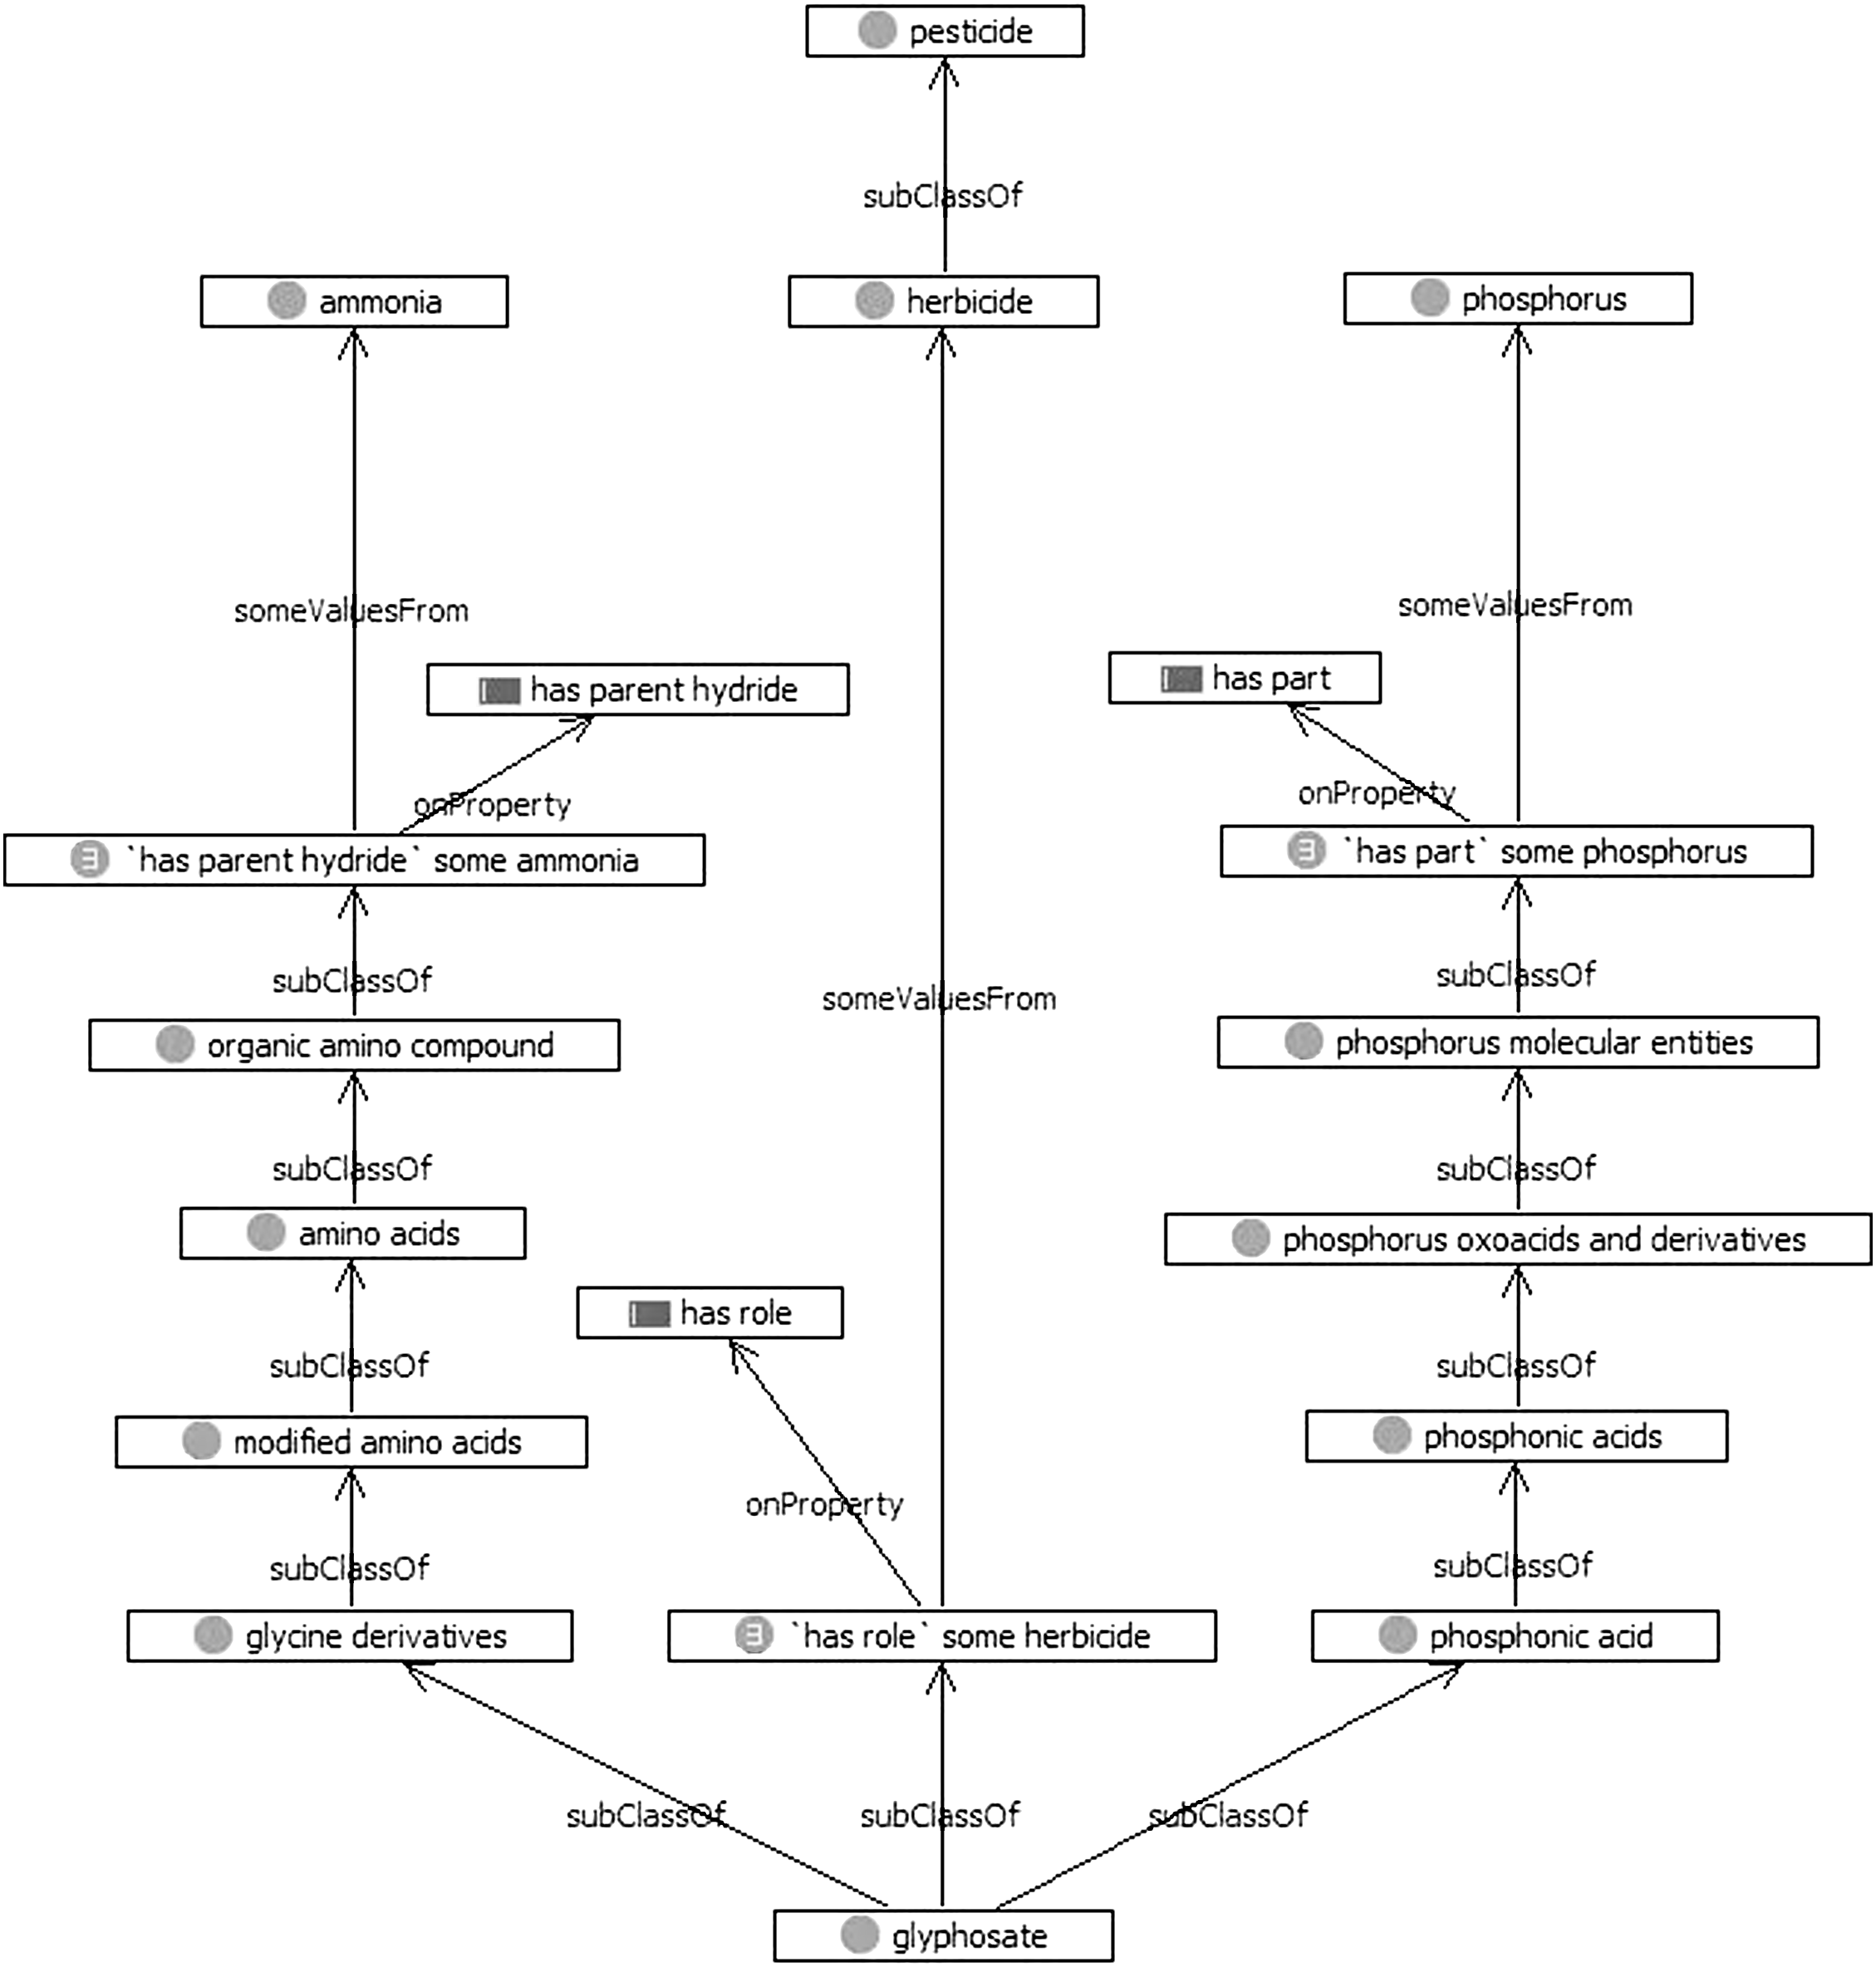
\includegraphics[width=5in]{media/ch14/f14-06.png}
\caption{Excerpt from CHEBI, showing information about glyphosate. All concepts
are shown with labels (e.g., ``glyphosate'') instead of CHEBI URIs
(e.g., \texttt{Chebi:CHEBI\_27744}).
}
\label{fig:ch14.06}
\end{figure}

Given these facts, we can use the inference mechanism of OWL to answer
some useful questions. Suppose we are interested in pesticides
containing phosphorus that have ammonia as a parent hydride. Figure
13.6, along with an understanding of the meaning of the modeling words
\texttt{rdfs:subClassOf}, \texttt{owl:someValuesFrom}, and \texttt{owl:onProperty} tells us that
glyphosate is such a chemical. But how, specifically, can we find this
(or any other such chemical), based on this model?

First, we define (in OWL) the class of things we are seeking, that is,
the intersection of things that have \textit{role} pesticide, have \textit{part}
phosphorus, and have \textit{parent hydride} ammonia. This is done with an
intersection of three restrictions. (In RDF, we have to use the CHEBI
URIs to refer to concepts; for reference, we have included the
corresponding names of the concepts pesticide, ammonia and
phosphorus in comments indicate with a hash (\#) on each line where they
occur.) Here's how that looks:

\begin{lstlisting}
:MyChemical a owl:Class ;
    rdfs:label "My chemical" ;
    owl:intersectionOf
       (
         [ a owl:Restriction ;
           owl:onProperty obo:has_role ;
	   owl:someValuesFrom chebi:CHEBI_25944 ] # pesticide
         [ a owl:Restriction ;
	   owl:onProperty obo:has_parent_hydride ;
	   owl:someValuesFrom chebi:CHEBI_16134 ] # ammonia
         [ a owl:Restriction ;
	   owl:onProperty obo:has_part ;
	   owl:someValuesFrom chebi:CHEBI_28659 ] # phosphorus
) .
\end{lstlisting}

Now if we run OWL inferences, we infer that

\begin{lstlisting}
chebi:CHEBI_27733 rdfs:subclassOf :MyChemical .
\end{lstlisting}

That is, \textit{glyphosate} is a match for the given specifications. The OWL
semantics took care of all the complexity of Figure~\ref{fig:ch14.06}, including the
chain of named classes that \textit{glyphosate} is a subclass of, as well as the
subclass chain between its stated role \textit{herbicide} and the required role
\textit{pesticide}. The definition of the requirements didn't include any
reference to any of these things---that was included in the CHEBI model
and the OWL semantics.

It is also worth noting what inferences we \textbf{\textit{cannot}} draw from the CHEBI
model as shown in Figure~\ref{14.06}. If, for example, we have a sample
chemical in our lab, and our experiments show that it contains
phosphorus as a part, and has ammonia as a parent hydride, this allows
us to infer its membership in the two corresponding restrictions at the
top of Figure~\ref{14.06}. But this does not allow us to infer anything about
the relationship of our sample to \textit{glyphosate}. CHEBI is useful for
searching for chemicals among those classified within it, not for
identifying samples.

These examples provide some motivation for why the authors of CHEBI
chose to define the
herbicide role of glyophosate as a relationship between classes using
someValuesFrom, rather than simply stating it as an explicit fact in a
single triple.

\begin{lstlisting}
chebi:CHEBI_27733 obo:has_role chebi:CHEBI_24527 .
\end{lstlisting}

By modeling this relationship with classes and \texttt{someValuesFrom}, they
embedded the class \textit{glyphosate} in a more comprehensive model that
includes relevant facts, for example, facts about the relations between
pesticides and herbicides. This allows the model (along with the OWL
semantics) to do a lot of the work of question answering (for certain
questions) about the entities in the model. The model encodes
information in a way that a human questioner need not be aware of.

\begin{challenge}{Expressing CHEBI in SKOS}
\label{chal:39}

The power of a model like CHEBI to respond flexibly to queries like this
one comes at a price---the model itself is complex; for example, the
relationship between \textit{glyphosate} and \textit{herbicide} is given by a pattern
including a particular kind of restriction. Earlier, we asked why this
couldn't have been represented simply with a single triple

\begin{lstlisting}
chebi:CHEBI_27733 obo:has_role chebi:CHEBI_24527 .
\end{lstlisting}

In this challenge, we will examine how CHEBI could be represented in
SKOS, and how we could satisfy the same information extraction needs
outlined above, using that representation.

In the case of CHEBI, it is a simple matter to convert all the
information about subclasses and restrictions into SKOS following this
line of reasoning. Each class in CHEBI becomes a SKOS concept, each
\texttt{rdfs:subClassOf} relationship becomes \texttt{skos:broader}, and each
\texttt{owl:someValuesFrom} restriction becomes a direct reference. Figure\ref{fig:ch14.07}
shows the same information from Figure~\ref{14.06}, but transformed into SKOS
in this way.

In many ways, Figure~\ref{14.07} is simpler than Figure Figure~\ref{14.06}; the fact that
glyphosate has role herbicide is represented as a single triple, as is
the fact that an organic amino compound has parent hydride ammonia. The
inclusion relationships that were expressed as \texttt{subClasbsof} are now
expressed as \texttt{broader}. But how would we query this structure to find an
answer to the same question we asked earlier---``find the pesticides
containing phosphorus that have ammonia as a parent hydride''? We can
find these using SPARQL as follows:

\begin{lstlisting}
SELECT ?result
WHERE {
  ?result skos:broader* ?concept1 .
  ?concept1 obo:has_parent_hydride ?concept2 .
  ?concept2 skos:broader* chebi:CHEBI_16134 . # ammonia
  ?result skos:broader* ?concept3 .
  ?concept3 obo:has_part ?concept4 .
  ?concept4 skos:broader* chebi:CHEBI_28659 . # phosphorus
  ?result skos:broader* ?concept5 .
  ?concept5 obo:has_role ?concept6 .
  ?concept6 skos:broader* chebi:CHEBI_25944 . # pesticide
}
\end{lstlisting}

This gives the same result as the OWL inference, namely that \textit{glyphosate}
satisfies all of these criteria. The representation is simpler, but the
query is more complex. In particular, the query writer must take
responsibility for all of the transitive relationships, using
\texttt{skos:broader*} at each point, and making sure that it appears at every
point in the query. This is a common trade-off in representation---does
the model do more work, with a more involved representation, or does the
query do more work, matching the correct information? The contrast
between the OWL version of CHEBI and the SKOS version shows this; in
OWL, certain queries can be done very easily, allowing the structure of
the model to do all the work. But the structure is less suited to other
queries (``Identify this sample''). The model does more of the work for
the queries it was designed for, but its increased complexity can make
other applications more complex.

The transformation from OWL into SKOS shown here was straightforward,
because CHEBI uses a single pattern (using \texttt{owl:someValuesFrom}) to relate
one concept to another. Some models use more complex pattern in OWL to
relate concepts. For instance, one of the OBO Foundry ontologies is a
thesaurus of cancer entities maintained by the National Cancer Institute
(NCI). The NCI thesaurus includes disease descriptions (with far too
much technical detail to include here) in which a disease is
characterized by several syndromes---that is, a particular disease is
indicated by a certain set of symptoms or another set of symptoms or
another set of symptoms and so on. Complicated combinations of unions
and intersections can be done in OWL in a standard way; the translation
to SKOS of such things is not straightforward. An OWL inference engine
will treat all such definitions in a consistent and correct manner.



\begin{figure}
\centering
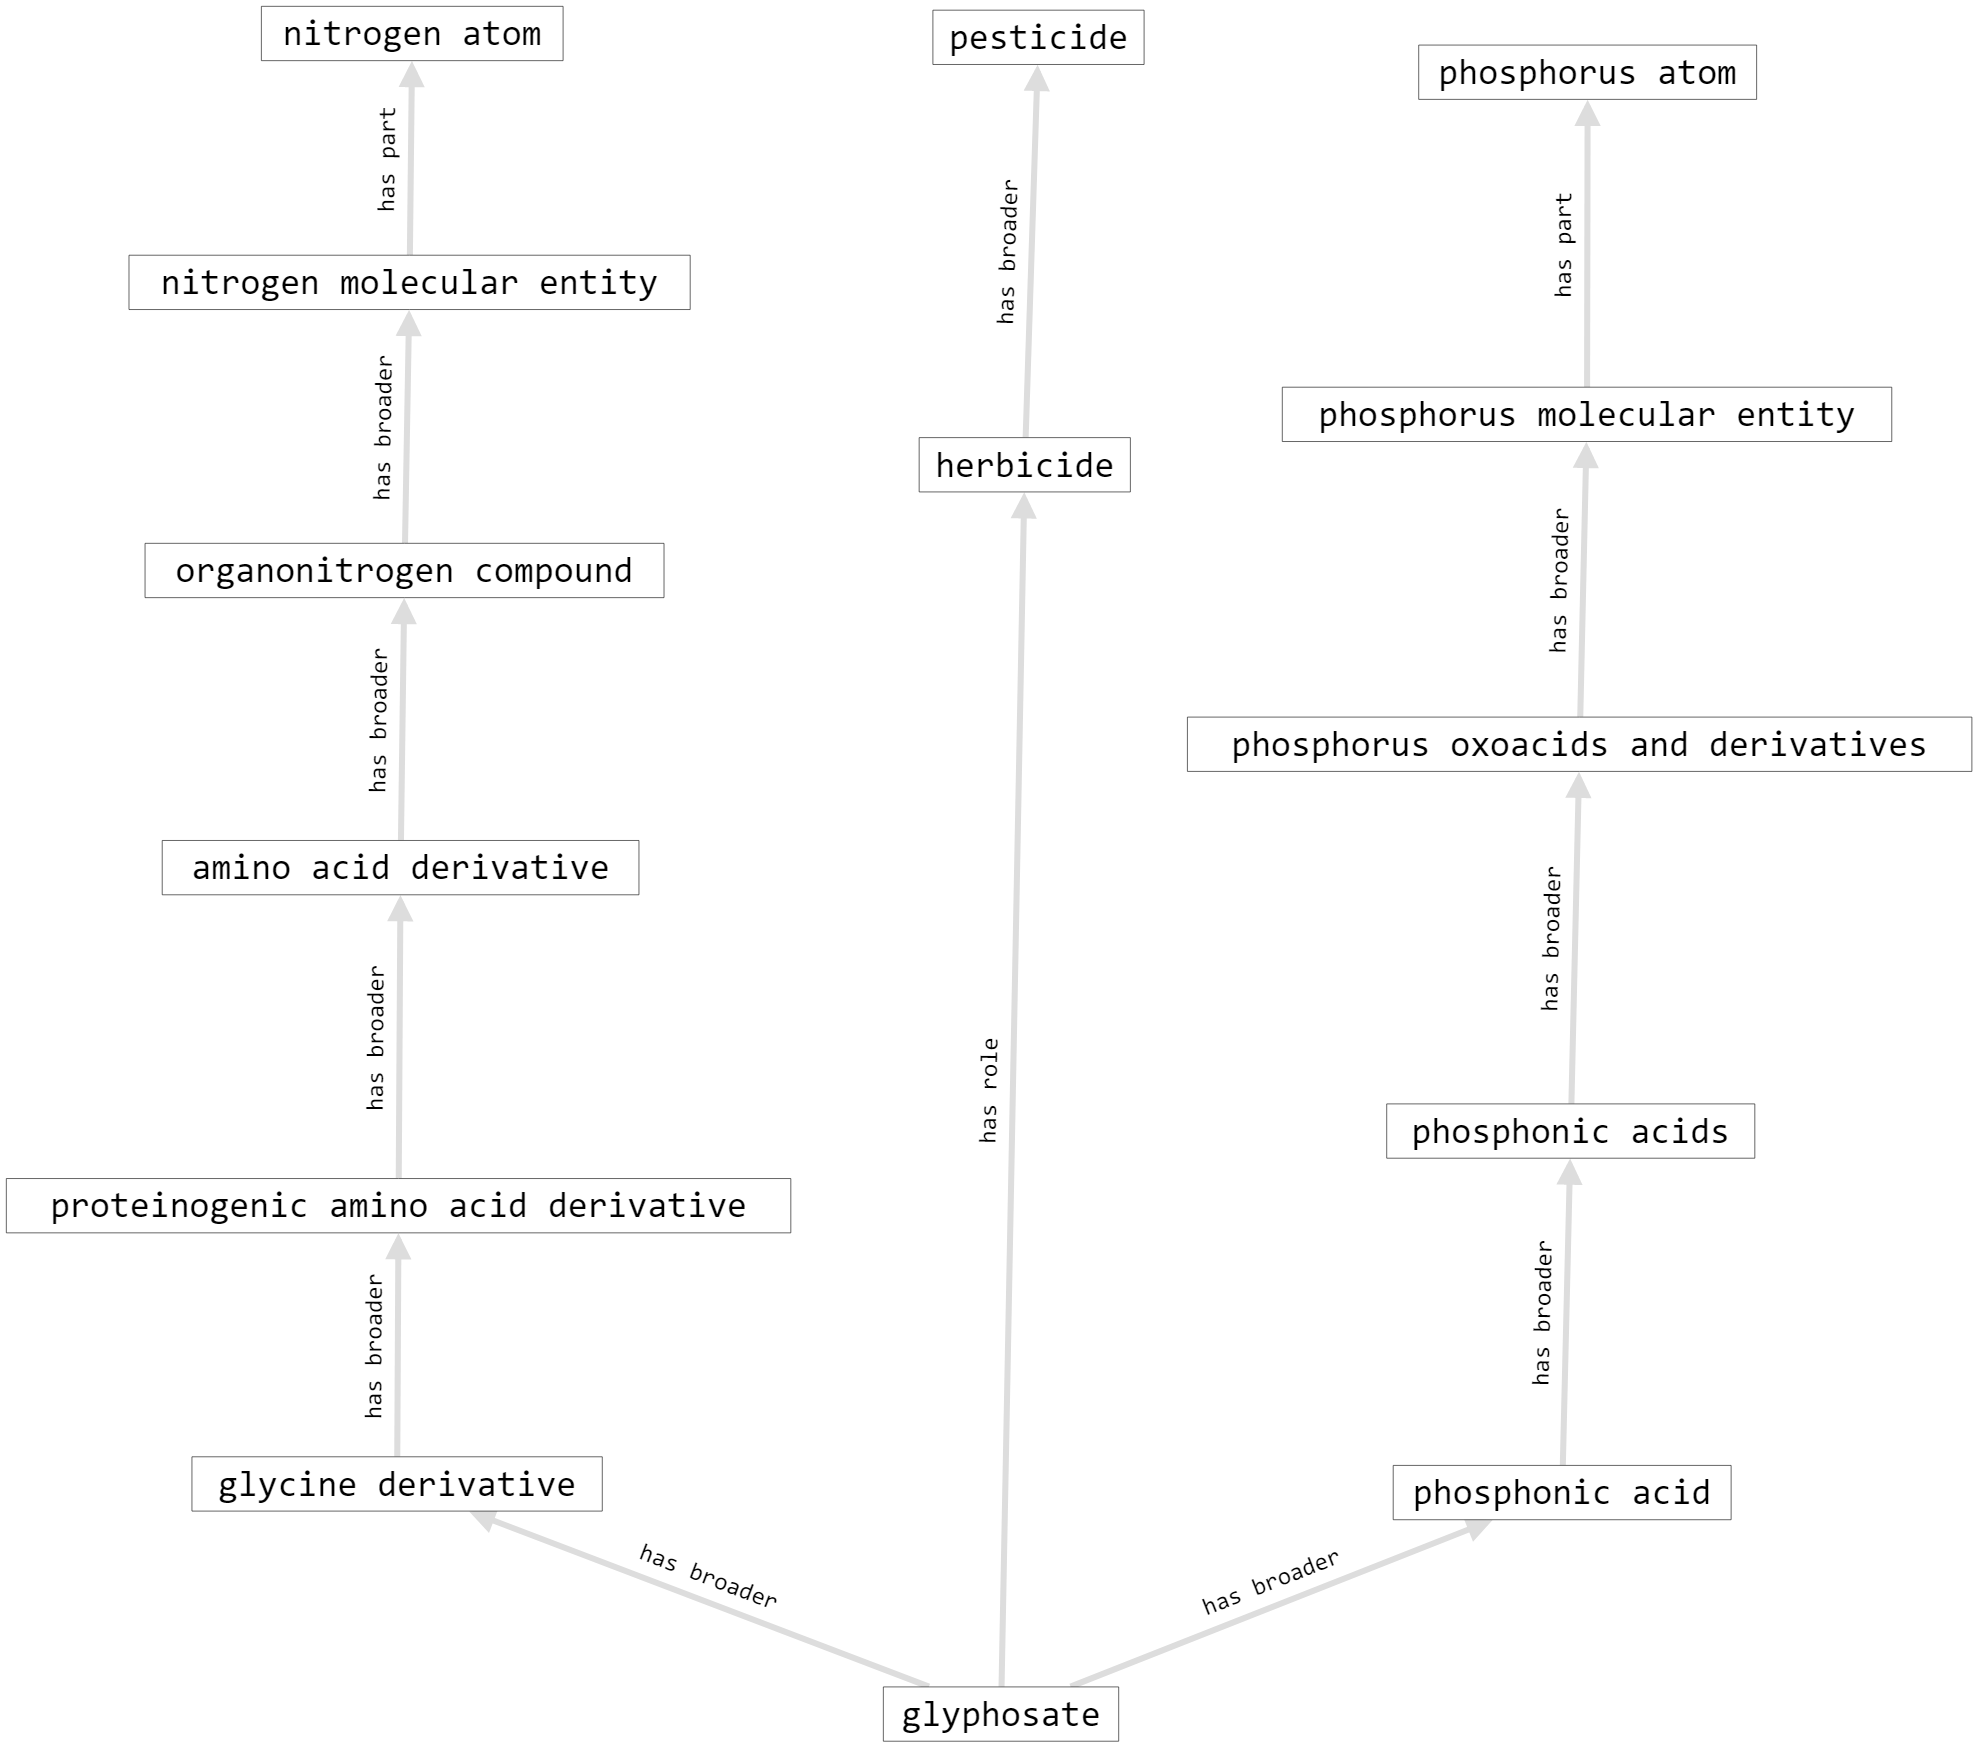
\includegraphics[width=5in]{SWWOv3/media/ch14/figure14-3.png}
\caption{CHEBI concepts from Figure \protect\ref{fig:ch14.06} shown in SKOS. The standard SKOS
property \texttt{skos:broader} is shown here as ``has broader.''
}
\label{fig:ch14.07}
\end{figure}
\end{challenge}

\section{FIBO - the Financial Industry Business Ontology}
\label{section:fibo}

FIBO is a massive undertaking to produce an ontology for describing financial instruments.  It is impossible to cover all aspects of FIBO 
in just a single chapter; more comprehensive details are available in the FIBO Primer,
\cite{fiboprimer}.   The industrial
motivation for FIBO is to make information about financial instruments more transparent at all levels. 
Specifically, 
FIBO assists in the following ways:

\begin{enumerate}
    \item Provide a means for financial institutions to report information in an interoperable way, so that regulators can 
    consume data from multiple providers and make sense of the aggregate, 
    \item Increase consistency in communication within and between financial institutions, 
    \item Encourage financial institutions to improve the quality of their own data management so that they have 
    more visibility into their own internal exposure, based on the instruments they participate in, and 
    \item Provide a starting point for institutions that want to manage all of the firm's information in an enterprise-wide knowledge graph. 
\end{enumerate}

\subsection{Modularity in FIBO}

Like Schema.org, FIBO is continually under development, responding to newly perceived needs by members of the 
finance industry.  At the time of this writing, FIBO includes over four thousand classes and nearly 2500 properties. As 
FIBO development continues, these numbers change. They don't always increase; it is possible for FIBO development to 
merge classes or properties so that the number will actually decrease as FIBO matures. 

These classes are organized into over 300 ontologies, taking the notion of ontology modularity to an extreme.  
For this reason, FIBO is organized into eleven \emph{domains} \footnote{FIBO Domains are not to be confused with \texttt{rdfs:domain}}
These domains are Foundations (FND), Business Entities (BE), Financial Business and Commerce (FBC), Loans (LOAN), Securities (SEC), 
Indices and Indicators (IND), and  Derivatives (DER).  Each of these domains has a short (2- to 4-letter) mnemonic.   With the exception of FND, which provides concepts that are useful across several industries, each domain covers a specific aspect of the
financial industry.

Naming so many ontologies can be a challenge.  FIBO meets this challenge by organizing each domain 
into \emph{sub-domains} and \emph{modules}. 
As we saw in Chapter~\ref{ch5}, HTTP URIs are expressive enough to represent arbitrary amounts of structure in names; 
FIBO takes advantage of this by reflecting the domains (and below domains, modules  and subdomains as needed) in the URI 
of each ontology.  For example, in the domain Business Entities, there is a module called \emph{Legal Entities}.  Inside that 
module, there are several ontologies, one of which is called \texttt{LegalPersons}.  The HTTP URI for this ontology
is made up of its complete heritage in FIBO, thus:

\begin{lstlisting}
https://spec.edmcouncil.org/fibo/ontology/BE/LegalEntities/LegalPersons/
\end{lstlisting}

FIBO implements the Follow-Your-Nose pattern (Section~\ref{dereferencing-http-uri}), so this HTTP URI resolves to 
a web resource that describes the ontology (try it in a web browser!). 

In FIBO, the definition of a resource can be distributed across a number of ontologies.  Each resource 
(i.e., Class, Property, Ontology or Individual) has a single ontology that is considered the ontology
that defines it.  The HTTP URI of the resource reflects the HTTP URI of its defining ontology.  For example,  the \texttt{LegalPersons}
ontology defines  a class called \texttt{BusinessEntity} whose HTTP URI is 

\begin{lstlisting}
https://spec.edmcouncil.org/fibo/ontology/BE/LegalEntities/LegalPersons/BusinessEntity
\end{lstlisting}

FIBO contains too many domains, subdomains, modules and ontologies to list all of them here. An index of all of them
is maintained by the EDM Council in a form called 
the \emph{fibopedia}\cite{fibopedia}.  

Since FIBO has hundreds of ontologies, it also has hundreds of namespace prefixes.  These are managed in a systematic way,
that corresponds to the systematic structure of the HTTP URIs themselves.  Not only does each FIBO domain have a short mnemonic, so 
does each subdomain and module.  These are concatenated together (with hyphens) to form namespace prefixes.  For example, the 
prefix for the LegalPersons ontology above is \texttt{fibo-be-le-lp:}.  Therefore, the CURIE for BusinessEntity 
is \texttt{fibo-be-le-lp:BusinessEntity}.  In the examples we'll show here, we will only use the official FIBO CURIEs, expanding
them out just once for each prefix. 

\subsection{FIBO and data mapping}

FIBO's main use case is data interoperability.  The financial institutions already manage structured data for their reference
data, instruments, positions, ratings, etc.  FIBO's job is to facilitate the exchange and comparison of this structured data. 
The challenge is that each data source is governed by a different organization, 
which will make different decisions about how to 
structure the data.  FIBO's approach to this challenge is to have a model 
to which each of these data sources can be mapped,  in advance of having seen the details 
of any of them.   At first blush, this might seem impossible; each of the 
data sources, not only from different parts of an organization, but 
from different organizations (e.g., banks, regulators, investors, credit card companies, 
tax agencies, etc.) is structured in a different way, 
and 
has been designed to emphasize a different use case, applications or
user group. 
How can one model 
possibly map to all of these things?

To see how FIBO meets this challenge, we need to understand the ways in 
which data sets from a variety of sources might differ.  
The first way is simply variation in naming.    
We saw several examples of this in Section~\ref{section:Equivalence}, where one
data set referred to an \emph{Analyst} whereas another 
data set referred to the same thing as a \emph{Researcher}, and in one 
library 
the patrons \emph{check out} the books whereas in another, 
they \emph{borrow} them.  

The second way that data sets from various sources might differ 
is more subtle, and we will call it \emph{factoring}.  
Even if we were to use the same names for all
the properties of the entities we describe, we could organize 
them differently.  For example, we could say that a credit card has
an address, or we could alternatively say that a credit card is 
held by a person (or company), and they have an address.  We could go further 
to say that a credit card has a billing zip code.  Or maybe the holder of 
the card has a billing address that has a zip code. 
An ontology like FIBO has to serve many masters, 
and be able to accommodate mapping to and from a wide variety of data sets. 

\begin{challenge}{Time periods}

Suppose we have a model that describes a period of time, 
with a start and an end.  We might model it like this: 

\begin{lstlisting}
:Period
  rdf:type owl:Class ;
:hasStart
  rdf:type owl:DatatypeProperty ;
  rdfs:domain :Period ;
  rdfs:range xsd:dateTime .
 
:hasEnd
  rdf:type owl:DatatypeProperty ;
  rdfs:domain :Period ;
  rdfs:range xsd:dateTime .
\end{lstlisting}

This provides a simple way to represent an interval of date/times. 

How can we map this to FIBO? 

\solution

FIBO defines a class called \texttt{fibo-fnd-dt-fd:DatePeriod}, defined as follows:

\begin{lstlisting}
fibo-fnd-dt-fd:DatePeriod
  rdf:type owl:Class ;
  rdfs:subClassOf [
      rdf:type owl:Restriction ;
      owl:maxQualifiedCardinality 1 ;
      owl:onClass fibo-fnd-dt-fd:Date ;
      owl:onProperty fibo-fnd-dt-fd:hasEndDate ] ;
  rdfs:subClassOf [
      rdf:type owl:Restriction ;
      owl:maxQualifiedCardinality 1 ;
      owl:onClass fibo-fnd-dt-fd:Date ;
      owl:onProperty fibo-fnd-dt-fd:hasStartDate ] .
\end{lstlisting}

In the challenge, the relationship between the class \texttt{Period} 
and the properties \texttt{hasStart} and \texttt{hasEnd} are 
given in RDFS, whereas in FIBO they are given in OWL.  
But the correspondence is direct; the meaning of \texttt{hasStart} 
is the same as 
the meaning for \texttt{fibo-fnd-dt-fd:hasStartDate}.  We can 
express this relationship in OWL as 

\begin{lstlisting}
fibo-fnd-dt-fd:hasStartDate owl:equivalentProperty :hasStart .
fibo-fnd-dt-fd:hasEndDate owl:equivalentProperty :hasEnd .
\end{lstlisting}
\end{challenge}


\begin{challenge}{Legal Entity Identifiers}

A common problem in the regulation of financial instruments 
is the identification of legal entities.  As a simple example, 
imagine that a stock brokerage firm owns an interest in many other 
companies.  A government regulation might say that they are 
forbidden from trading 
stocks in companies in which  they themselves own a significant share.  
How can we tell if this is the case?  We have to be able to 
identify the company that issued the stock that the brokerage 
is trading, and then look up to what extent the brokerage itself
owns part of the company. 

\solution

The finance industry approaches this problem by maintaining an 
identifier, called a \emph{Legal Entity Identifier} (or \emph{LEI} for short)
for companies in the world.  This identifier is a unique sequence of 
letters and digits and is quite long; for the examples in this 
example we will pretend that we have some short LEIs. 

One could imagine a simple data set that lists companies and 
their LEIs, modeled as in Figure~\ref{fig:ch14.simpleLEI}

\begin{figure}
\begin{lstlisting}
:Company a owl:Class .
:hasLEI a owl:DatatypeProperty ;
        rdfs:domain :Company ;
        rdfs:range xsd:string .

plush:BeautyBar :hasLEI "1234ABC" .        
\end{lstlisting}
    \caption{Simple model where every company has an LEI, and an example for the Plush Beauty Bar (see example \ref{Plushex})}
    \label{fig:ch14.simpleLEI}
\end{figure}


This is the sort of simple data representation you might expect 
in a spreadsheet or even in a Schema.org markup.  It allows you 
to look up an entity by its LEI. 

Now, let's imagine that instead of being a small company that  has 
registered an LEI and wants to inform its investors 
of it, we are looking at the data set that contains all of the LEIs in the 
world.  LEIs are managed by the 
\emph{Global LEI Foundation} (\emph{GLEIF} for short).  
They have a more elaborate representation of LEIs, as shown in 
Figure~\ref{fig:ch14.gleifLEI} \footnote{the GLEIF uses OWL to represent LEI registration, as published at 
www.gleif.org}

\begin{figure}
 \begin{lstlisting}
 gleif-L1:LegalEntityIdentifiera owl:Class ;
	rdfs:subClassOf
		[ a owl:Restriction ;
 		  owl:onProperty gleif-base:identifies ;
 		  owl:onClass gleif-L1:RegisteredEntity ;
 		  owl:qualifiedCardinality 1 ] .

gleif-base:Identifier a owl:Class ;
	rdfs:subClassOf
		[ a owl:Restriction ;
 		  owl:onProperty gleif-base:hasTag ;
 		  owl:onDataRange xsd:string ;
 		  owl:qualifiedCardinality 1 ] ,
		[ a owl:Restriction ;
 		  owl:onProperty gleif-base:identifies ;
 		  owl:cardinality 1 ] .

gleif-L1:RegisteredEntity a owl:Class .

plush:BeautyBar a gleif-L1:RegisteredEntity .
lei:L1234ABC a gleif-L1:LegalEntityIdentifier ;
             gleif-base:hasTag "1234ABC" ;
             gleif-base:identifies plush:BeautyBar . 
 \end{lstlisting}
    \caption{LEI structure as used by GLEIF, and an example of the Plush Beauty Bar}
    \label{fig:ch14.gleifLEI}
\end{figure}

One could well ask, why does the GLEIF have such a complex model 
for its identifiers, when clearly a much simpler one will do? 
The reason for this is that the GLEIF needs to know a lot more 
about its identifiers than just the entity identified and the number.
Since the GLEIF is managing the numbers, the model it uses also needs to be able to represent 
things about the number itself.  The GLEIF works with a number of
\emph{LOU}s, or \emph{Local Operating Units}, which are the entities that
have authority to issue LEIs.  From the GLEIF perspective, a model 
of the LEI has to be able to represent things about the LEI, in particular,  
which LOU it is registered with, which in turn, records other information such 
as payment for the registration (it costs a small fee to register an LEI and to 
renew it annually).  In short, 
from the GLEIF
perspective, the LEI itself plays a central role in the business, and needs to be
modeled separately from the entity it identifies. 
\end{challenge}


Where does FIBO come in to this?    FIBO can map fairly directly 
to the GLEIF model.  A relevant fragment of FIBO is given in 
Figure~\ref{fig:ch14.fibolei}

\begin{figure}
\begin{lstlisting}
fibo-be-le-lei:LegalEntityIdentifier
  a owl:Class ;
  rdfs:subClassOf fibo-fnd-arr-id:Identifier .
  rdfs:subClassOf [
      rdf:type owl:Restriction ;
      owl:onClass fibo-be-le-lp:LegalPerson ;
      owl:onProperty fibo-fnd-aap-agt:identifies ;
      owl:qualifiedCardinality 1 ] .
   
fibo-be-le-lei:LEIRegisteredEntity
  rdfs:subClassOf fibo-be-le-lp:LegalPerson ;
  owl:equivalentClass [
      rdf:type owl:Restriction ;
      owl:onProperty fibo-fnd-aap-agt:isIdentifiedBy ;
      owl:someValuesFrom fibo-be-le-lei:LegalEntityIdentifier ;
    ] .
  
fibo-fnd-arr-id:Identifier
  rdf:type owl:Class ;
  rdfs:subClassOf [
      rdf:type owl:Restriction ;
      owl:onDataRange xsd:string ;
      owl:onProperty fibo-fnd-rel-rel:hasTag ] 

plush:BeautyBar a fibo-be-le-lei:LEIRegisteredEntity .
plush:L1234ABC a fibo-be-le-lei:LegalEntityIdentifier ;
               fibo-fnd-rel-rel:hasTag "1234ABC" ;
               fibo-fnd-aap-agt:identifies plush:BeautyBar . 
\end{lstlisting}
    \caption{FIBO representation of Legal Entity Identifiers, Plush Beauty Bar as an example}
    \label{fig:ch14.fibolei}
\end{figure}

FIBO is already closely aligned to the model used by the 
GLEIF, but it has some differences.  This example shows one such difference. {the relevant parts of 
FIBO and GLEIF have been simplified for the purpose of this example, but the conclusions hold in the full 
models as well}
In the GLEIF model, the Beauty Bar is a Registered Entity, and no more inferences can be 
drawn from that fact (since \texttt{gleif-L1:RegisteredEntity} isn't a subclass of anything).  But in FIBO, 
the Beauty Bar is a \texttt{fibo-be-le-lei:LEIRegisteredEntity}, which, in turn, is a 
\texttt{fibo-be-le-lp:LegalPerson}.  In particular, in FIBO, a Legal Person has a liability capacity, that is
it can be sued at law.  The GLEIF model disagrees; there are some registered entities (in particular,
Branches and Funds) that are not legal persons, and therefore can not necessarily be sued.


This simple example shows the tightrope walk that FIBO faces; 
on the one hand, it has to answer questions like, "Does Plush 
have an LEI?  What is it?"
while managing the variation needed to satisfy regulators 
when someone asks, "Can the Plush Beauty Bar be sued at law?"  
A simpler model could answer
either of these questions, and indeed, simpler models are 
deployed on a regular basis to do so.  But when we want to 
integrate systems using those
simpler models, we need a model that encompasses all of the variation
of both models.  This is the main driving design rationale behind FIBO. 

\subsection{FIBO Summary}

FIBO has been designed to be a sort of ontological interlingua for 
data sets in the financial industry.  The examples here of Legal 
Entity Identification were chosen to be as simple as possible 
while illustrating the design challenges faced by such an ontology. 
A cursory examination of an ontology like FIBO could prompt 
the reader to wonder why there are so many pieces; for example, 
why is there 
a distinction between a \texttt{LEIRegisteredEntity} and a
\texttt{LegalEntity}?  What are the details of that distinction, and when
should 
I use one or the other? 

It is difficult to understand the design of an ontology like FIBO from the
viewpoint of use cases alone.  The main use case of FIBO is interoperability 
between data sets, and especially between data sets that we have not yet
encountered.  This means that FIBO has to \emph{anticipate} the structure of 
data sets in the finance industry, and provide abstractions that will match what
is natural for all of them.  In our simple example, one data
set (having to do with legal responsibility) is interested in the legal responsibility 
of an organization,
whereas another data set (the GLEIF's own management) is interested in how to
identify a corporation, without paying attention to its funding model
or status.  FIBO does not have the luxury of choosing one of these modes; its
job is to anticipate both of them, and to build a consistent 
model that incorporates them.


\section{SUMMARY}

The three ontologies discussed in this chapter, FIBO, QUDT,
and OBO Foundry ontologies, cover the spectrum from ontologies that
include very little data (FIBO) to ontologies that
include very large amounts of richly interconnected data (OBO). 
At the same time, they run from ontologies that say a lot about the 
structure of data (FIBO) to ontologies that say relatively little about 
it (OBO). 
They all
supply, to varying extents, the basic capabilities of the Semantic Web
of sharing information in a coherent way across multiple systems.

The job of FIBO is to describe how financial data can be interpreted and 
understood.  The data themselves, which could be details of a loan or a 
financial instrument, the price of a security on a certain day, 
or the standing of some account, are not part of the ontology at all, 
and are expected to be quite volatile and confidential.  Their structure, 
on the other hand, is quite complex and in many cases highly regulated. 

OBO Foundry
ontologies, in contrast, contain detailed data that describe particular 
chemicals.  The fact that glyphosate has a phosphate group is represented 
in CHEBI; nothing so specific is represented in FIBO. 
Some of the OBO ontologies are very large indeed, and contain massive
amounts of data about biology, medicine, life sciences, etc. There are
complex questions that can be answered, using OBO as a data resource.
QUDT sits in the middle; it contains a good deal of data (conversion
factors, relationships between dimensions and units, etc.), but its main
purpose is to provide connection between other data sets; two data
sources that both use FIBO might still fail to be
interoperable because of mismatch of units; QUDT provides enhanced
interoperability in these cases. All three of these ontologies play the
basic role in the Semantic Web of providing globally unambiguous names
for standard entities---they differ only in the details of how these
relationships can be used.

\subsection{Fundamental concepts}

The following fundamental concepts were introduced in this chapter.

owl:imports---Allows one ontology to refer explicitly to another.
Triples from the imported ontology are available for inferencing in the
importing ontology.

Ontology Design Patterns---Repeated modeling idioms that provide
coherence and unity to a large model.

Good Relations---Ontology for representing and sharing information about
commerce on the Web.

QUDT---Quantities, Units, Dimensions Types. Ontology of engineering
units

OBO---Open Biological and Biomedical Ontologies. A collection of
ontologies with relevance to the life sciences.

CHEBI---Chemical of Biological Interests. An example ontology from OBO
relating to biochemistry.
